\section{Methods}
\label{sec:methods}

\subsection{Unified evidence-evaluation design}

We evaluate one physical-proof requirement across two qualified atomistic source collections. Every claim is judged against the same types of evidence: stored-frame mobile and adsorbate displacement, rigid-aligned internal displacement, comparison identity, and permissible mathematical operations. The first collection establishes the effect of progressively stricter checks on fixed model selections. The second collection examines whether invalid proof selections persist with a different atomic source, an additional language model, and a separate output-format and confidence audit. Both collections use 16 base claims per source group in two evidence presentations, with matched representations and group-aware uncertainty analyses. Their output policies differ; therefore, pooled accuracy or a claimed direct replication of the first collection\'s check-ablation result would be inappropriate (Fig.~\ref{fig:workflow}).

\subsection{UMA-relaxed source collection and qualification}

The UMA collection tests whether a large language model (LLM) uses a physically compatible measurement to assess a claim. Initial structures were taken from the OC20-Dense validation set, which contains several placements of adsorbates on surfaces.\cite{chanussot2021open,lan2023adsorbml} Each source group represents one adsorbate--surface system. Twenty groups used during development were excluded before the final selection. The remaining groups and placements were ordered reproducibly using seed 20261021. One eligible placement was selected from each of 60 groups. Structures contained at most 180 atoms and at least three adsorbate atoms.

The structures were relaxed by adjusting atomic positions to reduce their forces. Forces came from the FAIRChem UMA \texttt{uma-s-1p2p1} checkpoint and its \texttt{oc20} task.\cite{wood2025uma} The Atomic Simulation Environment (ASE) FIRE optimizer was used with a time-step parameter of 0.1, a maximum step of 0.2~\AA, and a limit of 600 steps.\cite{larsen2017atomic} The cell and fixed surface atoms were held unchanged. Convergence required the largest force on a mobile atom to fall below 0.05~eV/\AA. Mobile atoms comprise the unfixed surface atoms and the adsorbate atoms.

Two runs did not converge. Three more changed the adsorbate distance graph and were excluded. This left 55 source groups. The graph connected two adsorbate atoms when their minimum-image distance was between 0.25~\AA{} and 1.25 times the sum of their ASE covalent radii. Qualification also required finite coordinates, unchanged atom identities and constraints, matching cells and periodic flags, and fixed-atom displacement no greater than 0.02~\AA. No excluded system was replaced. Close-contact and weak-contact annotations were retained as descriptive flags, rather than further exclusion rules. Each accepted endpoint also supplied a control made by translating only the adsorbate by 0.7~\AA{} along the stored $x$ direction. These controls supplied other-comparison evidence; they were not new relaxations.

\begin{center}
\begin{minipage}{\linewidth}
\centering
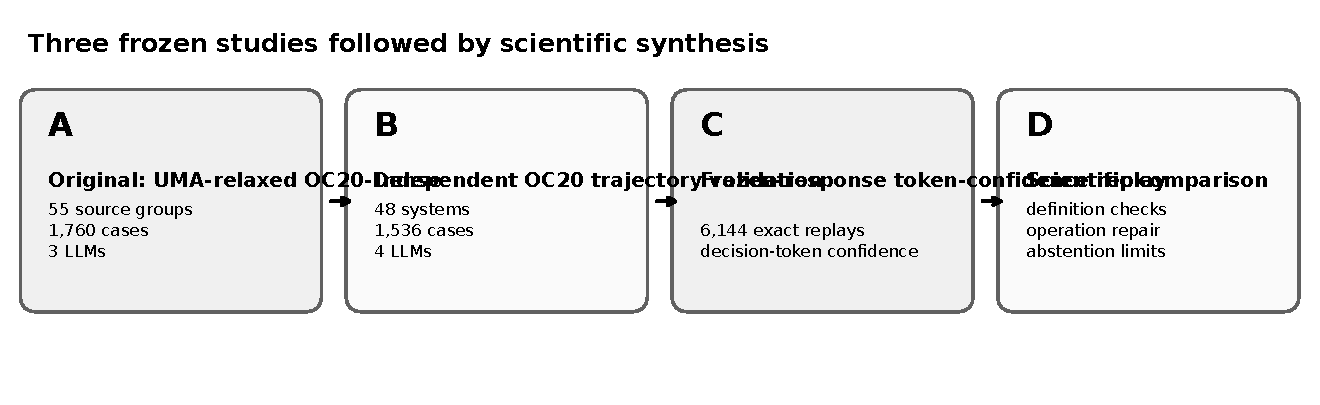
\includegraphics[width=\linewidth]{figure_01.pdf}
\captionof{figure}{One evidence-verification framework across UMA-relaxed and OC20 trajectory collections. The source-specific checks and confidence audit share physical definitions but retain their distinct scoring rules.}
\label{fig:workflow}
\end{minipage}
\end{center}

\subsection{RMSD definitions}

Root-mean-square deviation (RMSD) summarizes how far matched atoms differ between two structures. Its meaning depends on the selected atoms and the treatment of translation, rotation, and periodic boundaries. Atom correspondence was fixed throughout. For atom $i$, the displacement was
\begin{equation}
 \mathbf d_i=\operatorname{MIC}\!\left(\mathbf r_i^{(1)}-\mathbf r_i^{(0)}\right),
 \label{eq:displacement}
\end{equation}
Here, $i$ labels an atom, $\mathbf d_i$ is its displacement vector, and $\mathbf r_i^{(0)}$ and $\mathbf r_i^{(1)}$ are its initial and final positions. Periodic boundaries repeat the simulation cell. The function $\operatorname{MIC}$ selects the shortest equivalent displacement allowed by that cell. It was applied independently to each atom. The mobile-atom RMSD, $M$, and stored-frame adsorbate RMSD, $A$, were
\begin{equation}
 M=\left[\frac{1}{n_M}\sum_{i\in S_M}\|\mathbf d_i\|^2\right]^{1/2},
 \qquad
 A=\left[\frac{1}{n_A}\sum_{i\in S_A}\|\mathbf d_i\|^2\right]^{1/2}.
 \label{eq:frame}
\end{equation}
Here, $S_M$ and $S_A$ are the mobile and adsorbate atom sets, and $n_M$ and $n_A$ are their atom counts. The symbol $\|\cdot\|$ denotes vector length. Every atom received equal weight. Neither quantity removes molecular translation or rotation.

Internal RMSD, $I$, was calculated after the connected adsorbate was unwrapped at each endpoint. Unwrapping joins an adsorbate split across periodic boundaries into one connected image. The internal RMSD was
\begin{equation}
 I=\min_{\mathbf R,\mathbf t}
 \left[\frac{1}{n_A}\sum_{i\in S_A}
 \left\|\mathbf R\widetilde{\mathbf r}_i^{(0)}+\mathbf t
       -\widetilde{\mathbf r}_i^{(1)}\right\|^2\right]^{1/2}.
 \label{eq:internal}
\end{equation}
The positions $\widetilde{\mathbf r}_i^{(0)}$ and $\widetilde{\mathbf r}_i^{(1)}$ are the unwrapped coordinates. Here $\mathbf R$ is a rotation matrix, $\mathbf t$ is a translation vector, and $\min$ means we choose the pair that gives the smallest RMSD. A proper Kabsch rotation was used, which allows rotation but excludes reflection.\cite{kabsch1978discussion} No minimum-image correction was applied after fitting. All three RMSDs are reported in angstroms (\AA).

Because $S_A$ is a strict subset of $S_M$, their shared displacement convention gives
\begin{equation}
 M\geq A\sqrt{\frac{n_A}{n_M}},
 \qquad
 A\leq M\sqrt{\frac{n_M}{n_A}}.
 \label{eq:bounds}
\end{equation}
The bounds follow because the remaining mobile atoms add a nonnegative sum of squared displacements. They require the same comparison, frame, atom correspondence, periodic treatment, and equal weights. They do not provide a general bound between $I$ and $A$, which use different periodic and alignment procedures.

\subsection{Claims, evidence, and checking}

Each source group supplied 16 base claims. Each claim appeared as structured data and a short report. The final benchmark therefore contained 1,760 variants. Six base claims tested direct values, including unit conversion. Eight tested missing values using the bounds in Eq.~\ref{eq:bounds}. The last two supplied only fixed-atom evidence for missing internal RMSD, or evidence from another comparison. Thresholds were 0.75 or 1.25 times the relevant value or bound. These factors defined test cases, rather than chemical tolerances.

A claim was \emph{supported} when every value allowed by the evidence satisfied its inclusive inequality. It was \emph{contradicted} when every allowed value violated it. Otherwise, it had \emph{insufficient evidence}. The benchmark contained 550 supported, 550 contradicted, and 660 insufficient-evidence variants. The first two groups formed the 1,100 \emph{answerable cases}.

A \emph{licensed proof} was defined as one evidence record and one mathematical operation permitted by that record's physical definition. Operations could read a value, derive a mobile RMSD lower bound, or derive an adsorbate RMSD upper bound. Every alternative licensed proof was accepted. Generic relations were included in every prompt; the test did not require models to recall the bounds. Bound arithmetic used decimal precision of 50 digits. Coordinates and numerical cell vectors were not provided.

Evidence identifiers were replaced by neutral aliases, and records were shuffled. Both presentations retained the same numerical facts and physical definitions. The report presentation also removed redundant metric identifiers and display names. Thus, this comparison changed more than prose style alone.

\subsection{Model selection and proof-verification protocol}

The three models were Qwen3-4B-Instruct-2507, Phi-4-mini-instruct, and SmolLM3-3B, called Qwen, Phi, and SmolLM below. Each received two independent requests per variant. The \emph{direct-answer request} returned a scientific verdict, evidence identifier, and operation. The \emph{evidence-selection request} returned only the identifier and operation. Models had to follow a fixed JSON response format. One enclosing code-block wrapper was allowed; extra prose, unknown identifiers, invalid fields, and truncated responses were rejected without repair.

The same evidence selection was processed by three checks. The \emph{arithmetic-only check} applied the selected operation. The \emph{comparison-ID check} also required the requested comparison, meaning the specified pair of structures. The \emph{full-definition check} additionally required compatible atom sets, frame, alignment, periodic treatment, weights, and operation. No check searched for replacement evidence. A failed selection produced a \emph{workflow rejection}, which received no credit as scientific insufficiency. A separate \emph{deterministic oracle}, a program that tries every public record and permitted operation, established the task's solvability. All inference used one NVIDIA L40S GPU per model on UNL Swan. Generation used greedy decoding, which selects the most probable next token. Two requests were processed at a time using bfloat16 numerical precision. Each request allowed at most 160 new tokens and 6,144 input tokens. Inputs were not truncated. SmolLM extended thinking was disabled.

Direct-answer accuracy was measured both by verdict alone and by \emph{proof-aware accuracy}. The latter required a licensed proof for decisive claims or a correct explicit insufficiency response for insufficient claims. Valid numerical coverage was
\begin{equation}
 C=100\,\frac{N_{\mathrm{licensed}}}{N_{\mathrm{answerable}}}\;\%,
 \label{eq:coverage}
\end{equation}
where $C$ is the percentage of answerable cases answered correctly with a licensed proof. The counts $N_{\mathrm{licensed}}$ and $N_{\mathrm{answerable}}$ denote those valid answers and all answerable cases, respectively. Here, $N_{\mathrm{answerable}}=1{,}100$. An \emph{invalid acceptance} had either a wrong verdict or an unlicensed proof, even when its verdict happened to be correct.

Qwen was chosen during development for the primary comparison: full-definition versus comparison-ID checking on identical selections. Phi, SmolLM, and the presentation and task-family analyses were secondary. All 10,560 first attempts were retained, including malformed and output-cap failures. Uncertainty was estimated by resampling the 55 complete source groups 1,000 times (seed 20261021). All variants and paired conditions from a group remained together. Reported 95\% intervals are percentile intervals with linear interpolation and no multiple-testing adjustment. The protocol was fixed before final model inference, after development and source review; it was not externally preregistered.

\subsection{OC20 trajectory source collection and independent checks}
\label{sec:external_methods}

The complementary OC20 source collection uses the published OC20 IS2RE/IS2RS \texttt{val\_ood\_both} relaxation trajectories rather than the UMA-relaxed OC20-Dense systems in the original study.\cite{chanussot2021open} The original OC20 trajectory archive was downloaded and checked against its published MD5 digest. Each selected system supplies the first and last \emph{stored DFT relaxation frames}; we do not assume that the last stored frame reached a particular force tolerance or is a reference adsorption minimum. Independent hash ordering and predefined geometry qualification admitted 48 unique systems among the first 49 examined. This is a purposive qualified sample, not a random sample or a 48/49 acceptance-rate estimate for all OC20 trajectories.

The external geometry rules retain atom identity, surface-cell equality, periodic flags, and stationary fixed-atom constraints. The same shared-frame mobile RMSD ($M$), shared-frame adsorbate RMSD ($A$), and rigid-aligned internal RMSD ($I$) definitions are used as in Eqs.~\ref{eq:frame}--\ref{eq:bounds}. Each physical source pair also supplies one explicitly synthetic comparison control; those controls are not DFT relaxations. Each of 48 source groups contributes 16 base cases, each shown as structured evidence and as a written report. This gives 1,536 questions: 480 supported, 480 contradicted, and 576 insufficient-evidence cases. All valid one-record proof witnesses were sealed before external model inference; only public questions and evidence were sent to the models.

The external models are Qwen3-4B-Instruct-2507, Phi-4-mini-instruct, SmolLM3-3B, and Qwen3-32B-AWQ (4-bit weights). The 32B model is from the Qwen family and uses a different inference and quantization configuration; differences are not a controlled effect of parameter count. GPU generation was greedy with a 160-token output cap and 6,144-token input cap. Source groups were kept together across shards. The strict external score requires unfenced single-evidence JSON and a licensed conclusive proof on answerable cases. A separate diagnostic removes only an \emph{outer} Markdown JSON code fence; the model's evidence identifier, operation, and verdict are unchanged. The frozen operation-only repair checks an alternative permitted operation \emph{for the model-selected evidence identifier}; it is an oracle-assisted diagnostic ceiling, not a deployable inference method. When the complete public evidence and rules are available, the rule-only oracle enumerates all allowed proofs without any LLM selection.

\subsection{Confidence replay and statistical analysis}
\label{sec:confidence_methods}

The 1,536 external requests were replayed for each model with token probabilities recorded. All 6,144 replays reproduced the corresponding original answers exactly. We define \emph{decision-token confidence} as the geometric mean of conditional token probabilities for the chosen evidence identifier and mathematical operation. This token likelihood is \emph{not} interpreted as $P(\text{proof is correct})$. Confidence availability requires an unambiguous evidence identifier and operation; 42 answerable Phi cases and 225 answerable SmolLM cases had missing decision scores. We report those missing values, instead of imputing confidence. AUROC measures whether higher scores rank valid conclusive proofs above invalid ones on the 960 answerable cases per model; cases with insufficient evidence are analyzed separately. Within-model selective accuracy is measured by retaining the top 10\% of eligible answers. Uncertainty is descriptive, obtained by resampling complete OC20 source groups (48 clusters). These confidence outcomes are retrospective: the external correctness results had already been inspected, so no new untouched calibration or deployment threshold is claimed.